\section{Solution methods}
\label{sec:methods}

The set of methods we implemented, analysed and compared include: 
\begin{itemize}
	\item Deep Neural Network (DNN, see Section~\ref{sec:dnn}),
	\item Decision Tree (Section~\ref{sec:tree}),
	\item Support Vector Machine (SVM, Section~\ref{sec:svm}),
	\item $k$-Nearest Neighbours (\knn{}, Section~\ref{sec:knn}).	
\end{itemize}

Related work review shows that decision trees can achieve high 
accuracy results in arrhythmia classification based on ECG 
(electro-cardiogram) signals. 
As ECG and EGM representations are topologically close to each other, 
decision tree is a valid candidate for distinguishing fatal/non-fatal 
tachycardias based on EGMs.
Compared with neural networks, decision trees have an advantage that 
they are easy to interpret. 
Unlike neural network, the transparency of decision tree gives us a 
better understanding of the intermediate processes.
 
\knn{} algorithm is known for its implementation simplicity and fast 
training time. 
It is robust to noisy data, but sensitive to 
irrelevant features. 
The biggest disadvantage of \knn{} is its expensive computations in 
the testing phase. 
Moreover, in case of high-dimensional data, the distance between 
two data points becomes less meaningful and the accuracy may 
decrease~\cite{beyer1999nearest}. 

%PCA is a commonly used method to compress data and fasten 
%training process, and the data we will use is relatively large in 
%size (about 2MB per instance), so PCA could be useful, especially 
%when the model is not so simple, which requires a lot of calculation.

%After we complete the main part of our project,
%we also plan to show  beneficial results of applying Principal 
%Component 
%Analysis (PCA) for speeding up the performance. Though PCA is 
%usually used in unsupervised learning, we will show how it can be 
%applied to supervised learning algorithms such as DNN and SVM.  
%We will also focus on possible modifications of the algorithms such 
%as cost-sensitive decision tree, combining \knn{}, and
%AdaBoost. 

We used the following performance measures (See 
Section~\ref{sec:res}):
\begin{itemize}
	\item Accuracy (0-1 loss).
	\item Confusion matrix measures (TP, TN, FP, FN).
	\item Precision,  F1
	Sensitivity or 
	TPR ($\#$ correctly detected VT/$\#$ true VTs), 
	Specificity or 
	TNT ($\#$ correctly detected SVT/$\#$ true SVTs). 
	Those are very important performance measures in case of 
	tachycardia discrimination. Though FP (misclassifying SVT as VT) 
	might lead 	to a 	process of further examination or treatment 
	episodes which are 
	painful for the patient, FN (misclassifying VT as SVT) might put 
	the patient in the risk of death.  
	\item We also measured training 
	and test times.
%	\item Since PCA is used to reduce calculation costs, we will 
%	specifically 
%	measure how much training time was reduced after using PCA while 
%	test error is still above threshold. 
%	\item Since \knn{} is a memory-based algorithm we will report its 
%	test times. 
\end{itemize}
Now we will present each analysed approach in more details.

%\begin{figure*}[t]
%	\centering
%	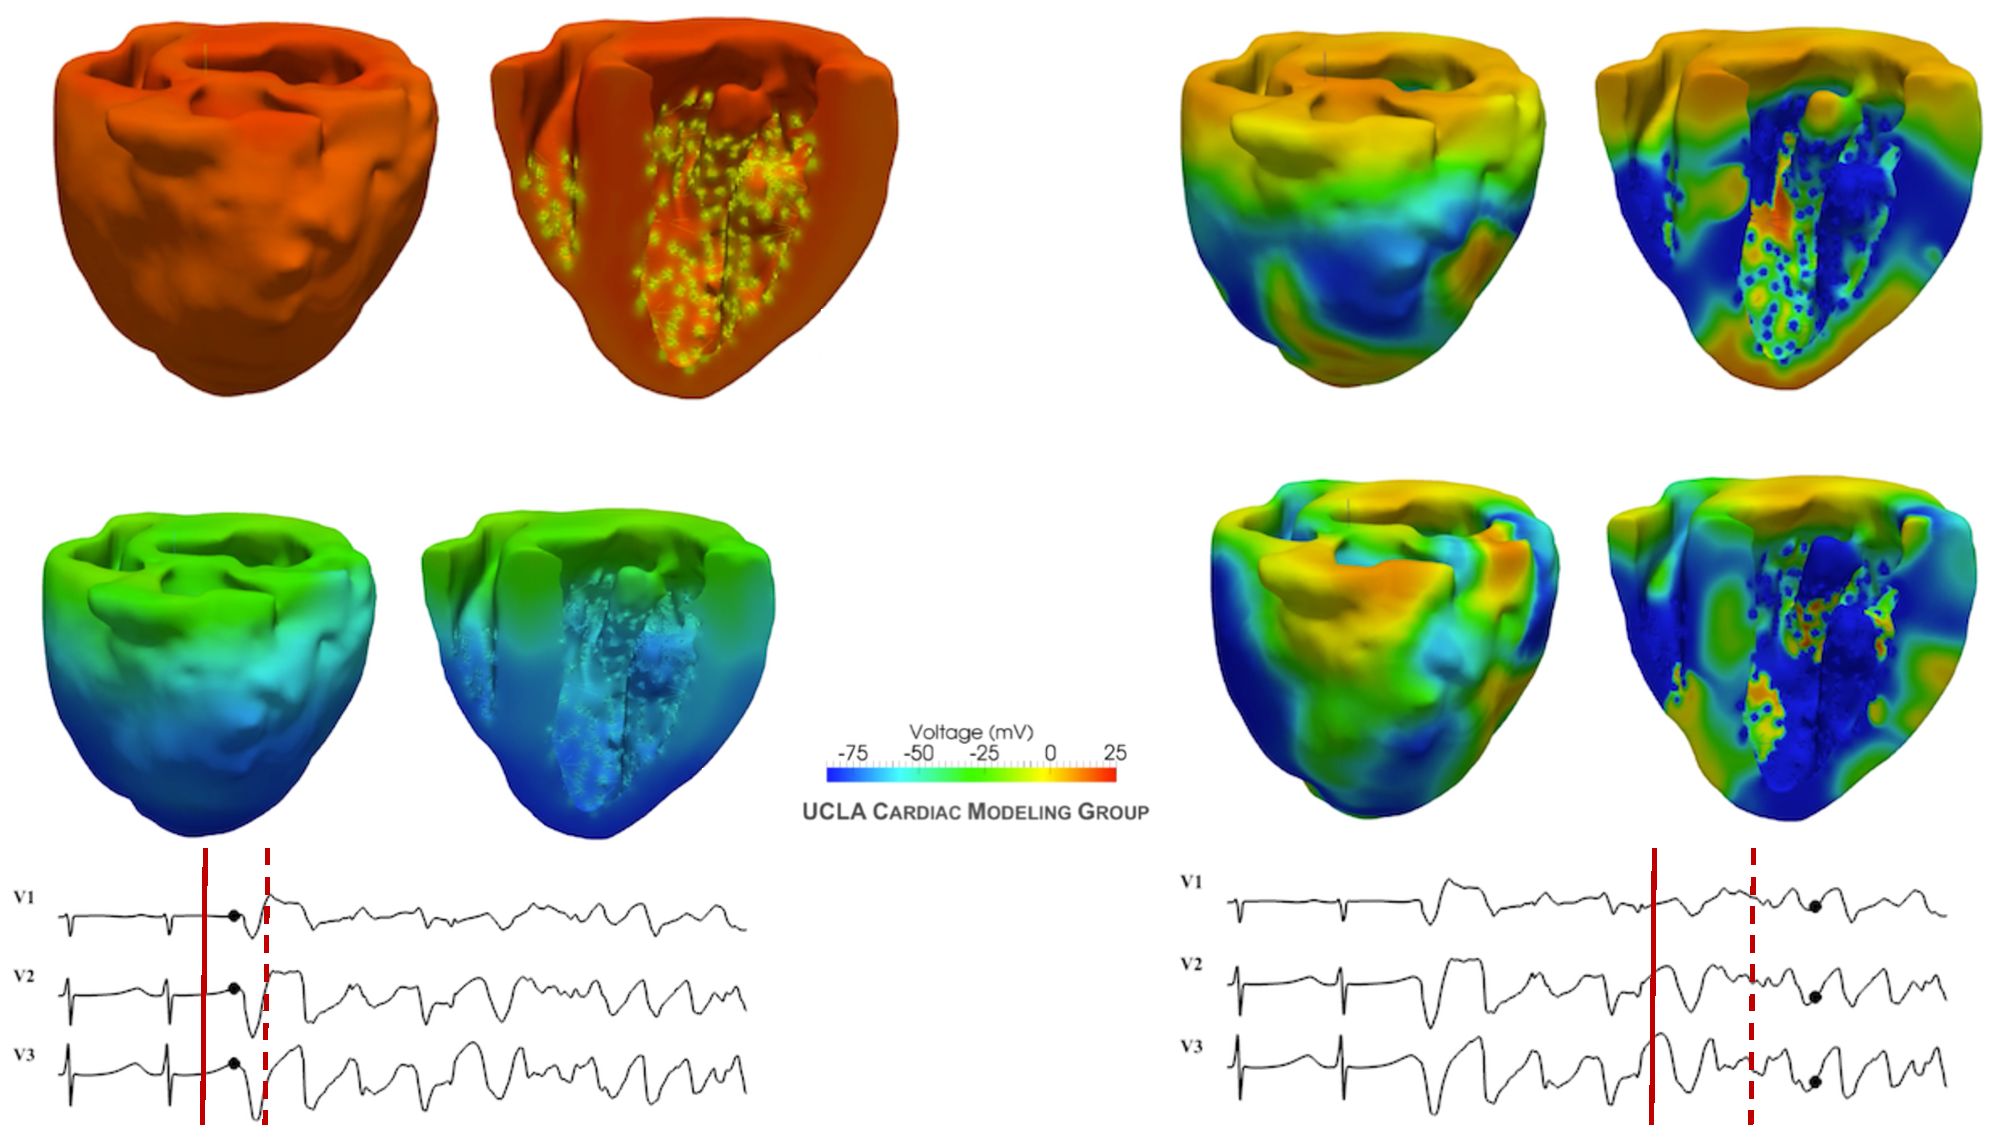
\includegraphics[width=0.9\linewidth]{figures/whnsrvfLowres.pdf}
%	\caption{Electrical activity during NSR and VF. The 
%	color scale runs from blue = rest state to red = excited (aka 
%	depolarized) state. (Colors in digital version).
%		In the top left, the ventricles are shown from two different 
%		angles, during a phase of NSR. The ventricles are fully 
%		exicted. The bottom left panel shows a later phase of the 
%		same beat, where the ventricles are progressively relaxing, 
%		starting with the apex (the pointed tip of the heart). This 
%		orderly propagation insures adequate muscle contraction and 
%		blood flow.
%		Three surface ECGs are shown beneath the left column, with 
%		red bars indicating the timing of the two snapshots. Note the 
%		periodic pattern.
%		The right column shows two snapshots during VF (earlier 
%		snapshot on top).
%		Note the disorganized nature of the electrical activity, 
%		wavefront breakup, and the multiple regions of 
%		depolarization. Note also the change in the surface ECG from 
%		periodic and regular (early on) to disorganized.
%		The AMA reads two such signals (obtained, however, 
%		intra-cardially and not from the surface) and tries to detect 
%		fibrillation. [Obtained from video of a simulation of the 
%		ventricles by the UCLA Cardiac Modeling Group, courtesy of 
%		Luigi Perrotti]}
%	\label{fig:whnsrvf}
%\end{figure*}